\documentclass[11pt,a4paper]{report}
\usepackage[textwidth=37em,vmargin=30mm]{geometry}
\usepackage{calc,xunicode,amsmath,amssymb,paralist,enumitem,tabu,booktabs,datetime2,xeCJK,xeCJKfntef,listings}
\usepackage{tocloft,fancyhdr,tcolorbox,xcolor,graphicx,eso-pic,xltxtra,xelatexemoji}

\newcommand{\envyear}[0]{2025}
\newcommand{\envdatestr}[0]{2025-01-24}
\newcommand{\envfinaldir}[0]{webdb/2025/20250124/final}

\usepackage[hidelinks]{hyperref}
\hypersetup{
    colorlinks=false,
    pdfpagemode=FullScreen,
    pdftitle={Web Digest - \envdatestr}
}

\setlength{\cftbeforechapskip}{10pt}
\renewcommand{\cftchapfont}{\rmfamily\bfseries\large\raggedright}
\setlength{\cftbeforesecskip}{2pt}
\renewcommand{\cftsecfont}{\sffamily\small\raggedright}

\setdefaultleftmargin{2em}{2em}{1em}{1em}{1em}{1em}

\usepackage{xeCJK,xeCJKfntef}
\xeCJKsetup{PunctStyle=plain,RubberPunctSkip=false,CJKglue=\strut\hskip 0pt plus 0.1em minus 0.05em,CJKecglue=\strut\hskip 0.22em plus 0.2em}
\XeTeXlinebreaklocale "zh"
\XeTeXlinebreakskip = 0pt


\setmainfont{Brygada 1918}
\setromanfont{Brygada 1918}
\setsansfont{IBM Plex Sans}
\setmonofont{JetBrains Mono NL}
\setCJKmainfont{Noto Serif CJK SC}
\setCJKromanfont{Noto Serif CJK SC}
\setCJKsansfont{Noto Sans CJK SC}
\setCJKmonofont{Noto Sans CJK SC}

\setlength{\parindent}{0pt}
\setlength{\parskip}{8pt}
\linespread{1.15}

\lstset{
	basicstyle=\ttfamily\footnotesize,
	numbersep=5pt,
	backgroundcolor=\color{black!5},
	showspaces=false,
	showstringspaces=false,
	showtabs=false,
	tabsize=2,
	captionpos=b,
	breaklines=true,
	breakatwhitespace=true,
	breakautoindent=true,
	linewidth=\textwidth
}






\newcommand{\coverpic}[2]{
    % argv: itemurl, authorname
    Cover photo by #2~~(\href{#1}{#1})
}
\newcommand{\makeheader}[0]{
    \begin{titlepage}
        % \newgeometry{hmargin=15mm,tmargin=21mm,bmargin=12mm}
        \begin{center}
            
            \rmfamily\scshape
            \fontspec{BaskervilleF}
            \fontspec{Old Standard}
            \fontsize{59pt}{70pt}\selectfont
            WEB\hfill DIGEST
            
            \vfill
            % \vskip 30pt
            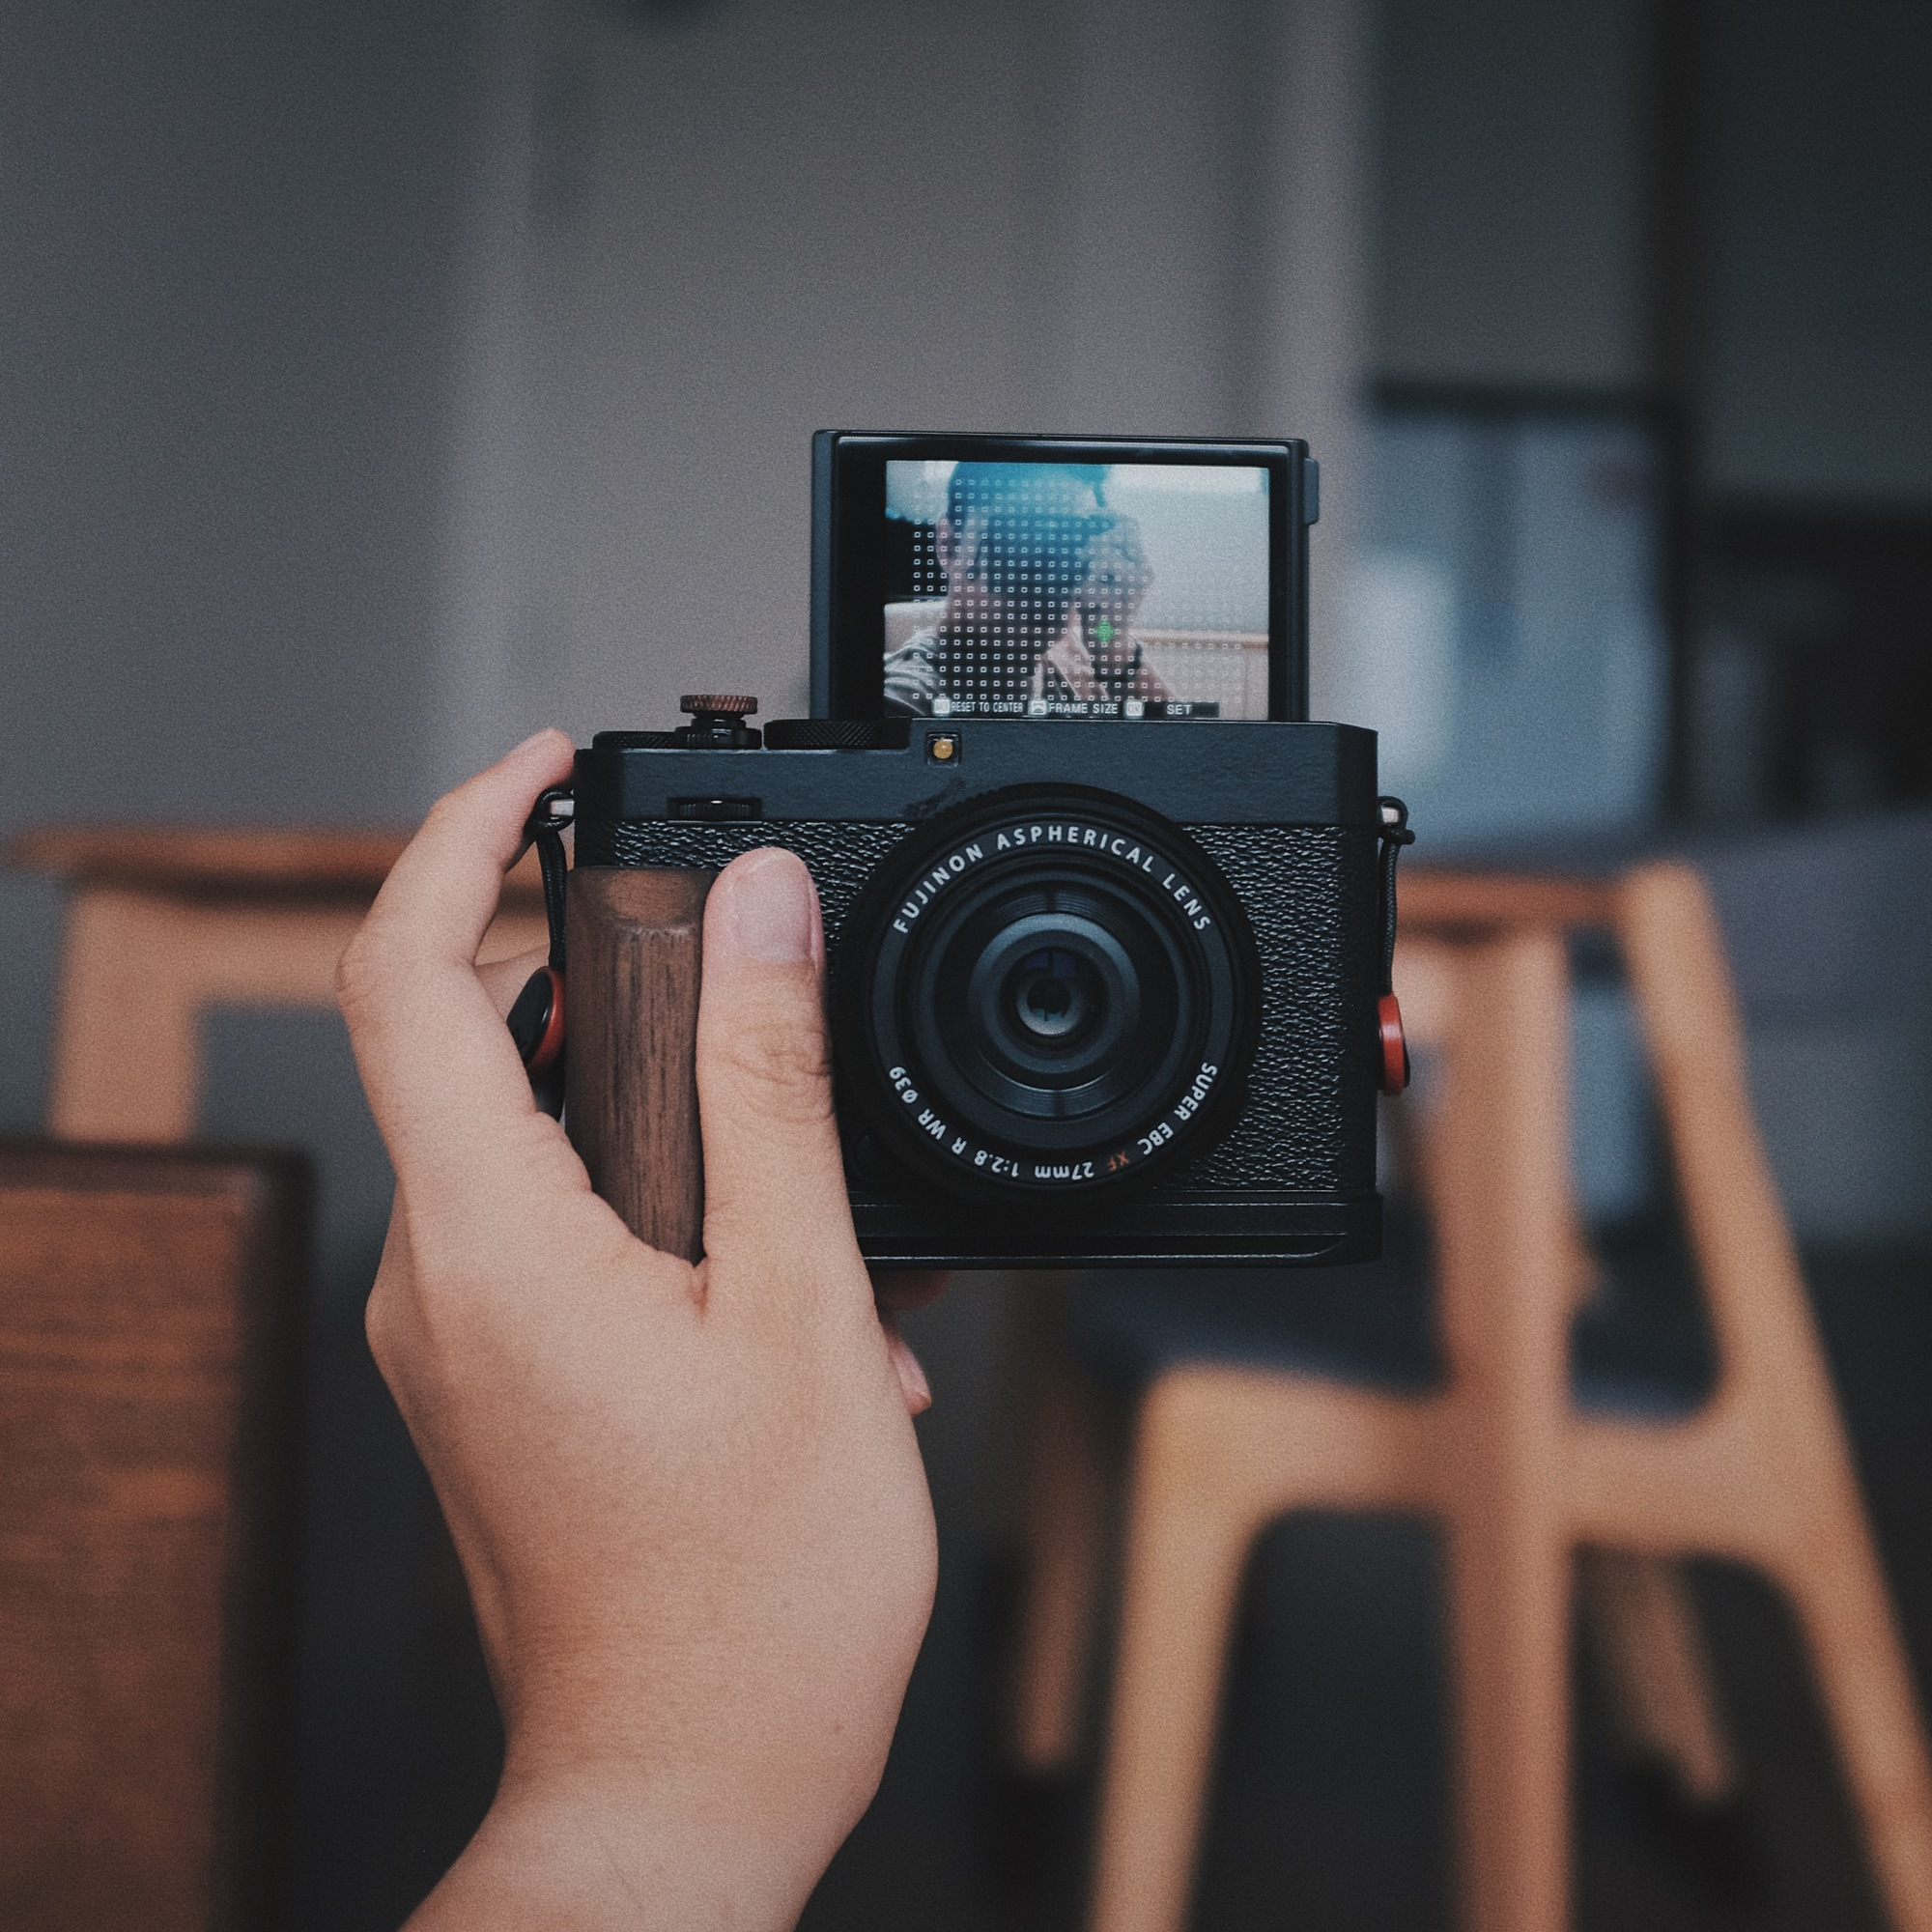
\includegraphics[width=\linewidth]{\envfinaldir/coverpic-prod.jpg}\par
            % \vskip 30pt
            \vfill

            \normalsize\rmfamily\scshape
            \copyright{} The Web Digest Project \hfill\large \envdatestr
        \end{center}
    \end{titlepage}
    % \restoregeometry
}
\newcommand{\simplehref}[1]{%
    \textcolor{blue!80!green}{\href{#1}{#1}}%
}
\renewcommand{\contentsname}{\center\Huge\sffamily\bfseries Contents\par\vskip 20pt}
\newcounter{ipartcounter}
\setcounter{ipartcounter}{0}
\newcommand{\ipart}[1]{
    % \vskip 20pt
    \clearpage
    \stepcounter{ipartcounter}
    \phantomsection
    \addcontentsline{toc}{chapter}{#1}
    % \begin{center}
    %     \Huge
    %     \sffamily\bfseries
    %     #1
    % \end{center}
    % \vskip 20pt plus 7pt
}
\newcounter{ichaptercounter}
\setcounter{ichaptercounter}{0}
\newcommand{\ichapter}[1]{
    % \vskip 20pt
    \clearpage
    \stepcounter{ichaptercounter}
    \phantomsection
    \addcontentsline{toc}{section}{\numberline{\arabic{ichaptercounter}}#1}
    \begin{center}
        \Huge
        \sffamily\bfseries
        #1
    \end{center}
    \vskip 20pt plus 7pt
}
\newcommand{\entrytitlefont}[1]{\subsection*{\raggedright\Large\sffamily\bfseries#1}}
\newcommand{\entryitemGeneric}[2]{
    % argv: title, url
    \parbox{\linewidth}{
        \entrytitlefont{#1}\par\vskip 5pt
        \footnotesize\ttfamily\mdseries
        \simplehref{#2}
    }\vskip 11pt plus 11pt minus 1pt
}
\newcommand{\entryitemGithub}[3]{
    % argv: title, url, desc
    \parbox{\linewidth}{
        \entrytitlefont{#1}\par\vskip 5pt
        \footnotesize\ttfamily\mdseries
        \simplehref{#2}\par\vskip 5pt
        \small\rmfamily\mdseries#3
    }\vskip 11pt plus 11pt minus 1pt
}
\newcommand{\entryitemAp}[3]{
    % argv: title, url, desc
    \parbox{\linewidth}{
        \entrytitlefont{#1}\par\vskip 5pt
        \footnotesize\ttfamily\mdseries
        \simplehref{#2}\par\vskip 5pt
        \small\rmfamily\mdseries#3
    }\vskip 11pt plus 11pt minus 1pt
}
\newcommand{\entryitemHackernews}[3]{
    % argv: title, hnurl, rawurl
    % \parbox{\linewidth}{
    %     \entrytitlefont{#1}\par\vskip 5pt
    %     \footnotesize\ttfamily\mdseries
    %     \simplehref{#3}\par
    %     \textcolor{black!50}{\href{#2}{#2}}
    % }\vskip 11pt plus 11pt minus 1pt
    \begin{minipage}{\linewidth}
            \entrytitlefont{#1}\par\vskip 5pt
            \footnotesize\ttfamily\mdseries
            \simplehref{#3}\par
            \textcolor{black!50}{\href{#2}{#2}}
    \end{minipage}\par\vskip 11pt plus 11pt minus 1pt
}







\begin{document}

\makeheader

\tableofcontents\clearpage




\ipart{Developers}
\ichapter{Hacker News}
\entryitemTwoLinks{Show HN: Open-source AI video editor}{https://news.ycombinator.com/item?id=42806616}{https://github.com/fal-ai-community/video-starter-kit}

\entryitemTwoLinks{Building a Medieval Castle from Scratch}{https://news.ycombinator.com/item?id=42806486}{https://www.guedelon.fr/en/}

\entryitemTwoLinks{Llama.vim – Local LLM-assisted text completion}{https://news.ycombinator.com/item?id=42806328}{https://github.com/ggml-org/llama.vim}

\entryitemTwoLinks{Introducing Operator}{https://news.ycombinator.com/item?id=42806301}{https://openai.com/index/introducing-operator/}

\entryitemTwoLinks{Thank HN: My bootstrapped startup got acquired today}{https://news.ycombinator.com/item?id=42806247}{https://news.ycombinator.com/item?id=42806247}

\entryitemTwoLinks{Working with Files Is Hard (2019)}{https://news.ycombinator.com/item?id=42805425}{https://danluu.com/deconstruct-files/}

\entryitemTwoLinks{Bunster: Compile bash scripts to self contained executables}{https://news.ycombinator.com/item?id=42804835}{https://github.com/yassinebenaid/bunster}

\entryitemTwoLinks{Psychedelic Graphics 0: Introduction}{https://news.ycombinator.com/item?id=42804566}{https://benpence.com/blog/post/psychedelic-graphics-0}

\entryitemTwoLinks{Turn any bicycle electric}{https://news.ycombinator.com/item?id=42804434}{https://dhruvvidyut.co.in/}

\entryitemTwoLinks{Shifting Cyber Norms: Microsoft security POST-ing to you}{https://news.ycombinator.com/item?id=42803597}{https://berthub.eu/articles/posts/shifting-cyber-norms-microsoft-post/}

\entryitemTwoLinks{Hacking Subaru: Tracking and Controlling Cars via the Starlink Admin Panel}{https://news.ycombinator.com/item?id=42803279}{https://samcurry.net/hacking-subaru}

\entryitemTwoLinks{The British Micro Behemoth}{https://news.ycombinator.com/item?id=42802778}{https://www.abortretry.fail/p/the-british-micro-behemoth}

\entryitemTwoLinks{Where is London's most central sheep?}{https://news.ycombinator.com/item?id=42802498}{https://diamondgeezer.blogspot.com/2025/01/londons-most-central-sheep.html}

\entryitemTwoLinks{Bun 1.2 Is Released}{https://news.ycombinator.com/item?id=42801370}{https://bun.sh/blog/bun-v1.2}

\entryitemTwoLinks{Show HN: I built an active community of trans people online}{https://news.ycombinator.com/item?id=42800893}{https://t4t.social/}

\entryitemTwoLinks{Tech takes the Pareto principle too far}{https://news.ycombinator.com/item?id=42800557}{https://bobbylox.com/blog/tech-takes-the-pareto-principle-too-far/}

\entryitemTwoLinks{Foundations of Large Language Models}{https://news.ycombinator.com/item?id=42799629}{https://arxiv.org/abs/2501.09223}

\entryitemTwoLinks{Show HN: I organized Bluesky feeds by categories and growth rankings}{https://news.ycombinator.com/item?id=42799574}{https://www.bskyinfo.com/feeds/}

\entryitemTwoLinks{Trae: An AI-powered IDE by ByteDance}{https://news.ycombinator.com/item?id=42799540}{https://www.trae.ai/home}

\entryitemTwoLinks{Understanding gRPC, OpenAPI and REST and when to use them in API design (2020)}{https://news.ycombinator.com/item?id=42799245}{https://cloud.google.com/blog/products/api-management/understanding-grpc-openapi-and-rest-and-when-to-use-them}\ichapter{Phoronix}
\entryitemGeneric{\hskip 0pt{}x86 32-bit Operating Systems Aren't Dead Yet: New Linux Patches Improve 32-bit PAE}{https://www.phoronix.com/news/Linux-2025-Improving-32-bit-PAE}

\entryitemGeneric{\hskip 0pt{}KDE Plasma 6.3 Beta 2 Improves systemd-homed Support}{https://www.phoronix.com/news/KDE-Plasma-6.3-Beta-2}

\entryitemGeneric{\hskip 0pt{}Linux 6.14 Power Management: "Dominated By AMD P-State Driver Changes"}{https://www.phoronix.com/news/Linux-6.14-Power-Management}

\entryitemGeneric{\hskip 0pt{}Redis 8.0-M3 Brings Async I/O Threading, 12x Speed-Up With New AVX2 Code Path}{https://www.phoronix.com/news/Redis-8.0-M3-Async-IO-Threads}

\entryitemGeneric{\hskip 0pt{}Debian 15 Is Codenamed "Duke"}{https://www.phoronix.com/news/Debian-15-Duke}

\entryitemGeneric{\hskip 0pt{}NVIDIA GeForce RTX 5090 Linux Benchmarks: Stay Tuned}{https://www.phoronix.com/news/GeForce-RTX-5090-Linux-Driver}

\entryitemGeneric{\hskip 0pt{}Faster AES-GCM \& AES-XTS Crypto Performance For AMD CPUs With Linux 6.14}{https://www.phoronix.com/news/Linux-6.14-Crypto}

\entryitemGeneric{\hskip 0pt{}Linux 6.14 Adds Support For The Microsoft Copilot Key Found On New Laptops}{https://www.phoronix.com/news/Linux-6.14-Input}

\entryitemGeneric{\hskip 0pt{}Red Hat Preparing Tuned 2.25 Daemon For Linux Monitoring \& Adaptive Performance Tuning}{https://www.phoronix.com/news/Red-Hat-Tuned-2.25-RC}\ichapter{Dribbble}
\entryitemGeneric{\hskip 0pt{}Carbon Solutions B2B Dashboard Design}{https://dribbble.com/shots/25506638-Carbon-Solutions-B2B-Dashboard-Design}

\entryitemGeneric{\hskip 0pt{}Goose Gym}{https://dribbble.com/shots/25515121-Goose-Gym}

\entryitemGeneric{\hskip 0pt{}HappyDev - Logo Design / Branding}{https://dribbble.com/shots/25514894-HappyDev-Logo-Design-Branding}

\entryitemGeneric{\hskip 0pt{}The Toucan}{https://dribbble.com/shots/25515890-The-Toucan}

\entryitemGeneric{\hskip 0pt{}Rapid Rabbit Logo}{https://dribbble.com/shots/25516738-Rapid-Rabbit-Logo}

\entryitemGeneric{\hskip 0pt{}VCC Unused Logo Design Concept}{https://dribbble.com/shots/25511334-VCC-Unused-Logo-Design-Concept}

\entryitemGeneric{\hskip 0pt{}LLM GPU Manager}{https://dribbble.com/shots/25513811-LLM-GPU-Manager}

\entryitemGeneric{\hskip 0pt{}Bestest Brand®}{https://dribbble.com/shots/25510300-Bestest-Brand}

\entryitemGeneric{\hskip 0pt{}QVELTY / Design \& Animation}{https://dribbble.com/shots/25507639-QVELTY-Design-Animation}

\entryitemGeneric{\hskip 0pt{}Haptic Logo Design}{https://dribbble.com/shots/25504012-Haptic-Logo-Design}

\entryitemGeneric{\hskip 0pt{}Wine Label}{https://dribbble.com/shots/25509757-Wine-Label}

\entryitemGeneric{\hskip 0pt{}Letter V + LED + Wires Logo}{https://dribbble.com/shots/25507506-Letter-V-LED-Wires-Logo}

\entryitemGeneric{\hskip 0pt{}Robin bird logo}{https://dribbble.com/shots/25509208-Robin-bird-logo}

\entryitemGeneric{\hskip 0pt{}Qore - Logo Design}{https://dribbble.com/shots/25509466-Qore-Logo-Design}

\entryitemGeneric{\hskip 0pt{}Wine Label}{https://dribbble.com/shots/25503830-Wine-Label}

\entryitemGeneric{\hskip 0pt{}Monocle Cat}{https://dribbble.com/shots/25502155-Monocle-Cat}

\entryitemGeneric{\hskip 0pt{}Roundrobin}{https://dribbble.com/shots/25502404-Roundrobin}

\entryitemGeneric{\hskip 0pt{}"Nature Morte" - Promotional piece}{https://dribbble.com/shots/25501105--Nature-Morte-Promotional-piece}

\entryitemGeneric{\hskip 0pt{}Fitness App Design}{https://dribbble.com/shots/25494068-Fitness-App-Design}

\entryitemGeneric{\hskip 0pt{}404}{https://dribbble.com/shots/25492419-404}

\entryitemGeneric{\hskip 0pt{}Personal Banking App}{https://dribbble.com/shots/25493958-Personal-Banking-App}

\entryitemGeneric{\hskip 0pt{}Wine Label}{https://dribbble.com/shots/25490604-Wine-Label}

\entryitemGeneric{\hskip 0pt{}planet}{https://dribbble.com/shots/25490310-planet}

\entryitemGeneric{\hskip 0pt{}Shihiko // E-commerce Website}{https://dribbble.com/shots/25489208-Shihiko-E-commerce-Website}


\ipart{Developers~~~~(zh-Hans)}
\ichapter{Solidot}
\entryitemGeneric{\hskip 0pt{}万事达卡 DNS 错误存在了五年之久}{https://www.solidot.org/story?sid=80405}

\entryitemGeneric{\hskip 0pt{}Debian 13.0 Trixie 预计今年夏天发布}{https://www.solidot.org/story?sid=80404}

\entryitemGeneric{\hskip 0pt{}Telegram 屏蔽 RuTracker 频道}{https://www.solidot.org/story?sid=80402}

\entryitemGeneric{\hskip 0pt{}在出售给美国买家前苹果应用商店不会重新上架 TikTok}{https://www.solidot.org/story?sid=80400}

\entryitemGeneric{\hskip 0pt{}过去一个世纪男性身高体重增长速度两倍于女性}{https://www.solidot.org/story?sid=80399}

\entryitemGeneric{\hskip 0pt{}杭州深度求索发布能挑战 OpenAI o1 的推理模型 DeepSeek R1}{https://www.solidot.org/story?sid=80398}

\entryitemGeneric{\hskip 0pt{}黑猩猩的撒尿行为具有传染性}{https://www.solidot.org/story?sid=80397}

\entryitemGeneric{\hskip 0pt{}耐药菌在乌克兰扩散}{https://www.solidot.org/story?sid=80396}

\entryitemGeneric{\hskip 0pt{}中国 2024 年可更新能源装机容量再创记录}{https://www.solidot.org/story?sid=80395}

\entryitemGeneric{\hskip 0pt{}Wine 10.0 释出}{https://www.solidot.org/story?sid=80394}

\entryitemGeneric{\hskip 0pt{}TikTok 被指限制反特朗普关键词的搜索}{https://www.solidot.org/story?sid=80393}

\entryitemGeneric{\hskip 0pt{}IMDb 创始人卸任 CEO 一职}{https://www.solidot.org/story?sid=80392}

\entryitemGeneric{\hskip 0pt{}特朗普赦免 Ross Ulbricht}{https://www.solidot.org/story?sid=80391}

\entryitemGeneric{\hskip 0pt{}北京将举办首届人机马拉松}{https://www.solidot.org/story?sid=80390}

\entryitemGeneric{\hskip 0pt{}X、Facebook、Instagram 和 YouTube 向欧盟承诺处理仇恨言论}{https://www.solidot.org/story?sid=80389}

\entryitemGeneric{\hskip 0pt{}干旱愈来愈严重愈来愈频繁}{https://www.solidot.org/story?sid=80388}

\entryitemGeneric{\hskip 0pt{}愈来愈多的美国青少年使用 ChatGPT 完成作业 }{https://www.solidot.org/story?sid=80387}

\entryitemGeneric{\hskip 0pt{}Paul Allen 诞辰 72 周年}{https://www.solidot.org/story?sid=80386}

\entryitemGeneric{\hskip 0pt{}孕妇的脑灰质在孕期发生变化}{https://www.solidot.org/story?sid=80385}

\entryitemGeneric{\hskip 0pt{}佳能的直播应用不支持佳能摄像机}{https://www.solidot.org/story?sid=80384}\ichapter{V2EX}
\entryitemGeneric{\hskip 0pt{}[程序员] 腾讯医典的静态服务被滥用?}{https://www.v2ex.com/t/1107466}

\entryitemGeneric{\hskip 0pt{}[问与答] 有个闲置 16G 显卡能拿来做什么?}{https://www.v2ex.com/t/1107465}

\entryitemGeneric{\hskip 0pt{}[问与答] 小红书刷的时间越长推荐内容质量越差}{https://www.v2ex.com/t/1107463}

\entryitemGeneric{\hskip 0pt{}[问与答] 为什么帖子发了后移动节点后看不到}{https://www.v2ex.com/t/1107462}

\entryitemGeneric{\hskip 0pt{}[职场话题] 技术人员受到不公平待遇也不是国内独有的事情}{https://www.v2ex.com/t/1107461}

\entryitemGeneric{\hskip 0pt{}[问与答] app store 现在充值 9 折优惠的活动能续费 688 开发者证书不?}{https://www.v2ex.com/t/1107459}

\entryitemGeneric{\hskip 0pt{}[游戏] 25 年二月份似乎有不少游戏新续作}{https://www.v2ex.com/t/1107458}

\entryitemGeneric{\hskip 0pt{}[程序员] 有没有什么提升开发生产力的订阅推荐啊? PS:已经有 GPT 和 Cursor 了}{https://www.v2ex.com/t/1107457}

\entryitemGeneric{\hskip 0pt{}[Podcast] 那种没说几句就开始哈哈大笑的小圈子文化播客,为何受众一点不少?}{https://www.v2ex.com/t/1107456}

\entryitemGeneric{\hskip 0pt{}[程序员] 51la 统计疑似又开始劫持跳转了}{https://www.v2ex.com/t/1107455}

\entryitemGeneric{\hskip 0pt{}[程序员] 求助,如何排查 chrome 被 360 劫持新姿势}{https://www.v2ex.com/t/1107454}

\entryitemGeneric{\hskip 0pt{}[宽带症候群] 请教 UU 加速器路由器插件和 mihomo tun 模式该怎么兼容}{https://www.v2ex.com/t/1107453}

\entryitemGeneric{\hskip 0pt{}[问与答] 最近 github 搜不到关于某东 某宝的签到任务脚本仓库了}{https://www.v2ex.com/t/1107452}

\entryitemGeneric{\hskip 0pt{}[问与答] 新号 新手机号如何尽量避免被电话骚扰}{https://www.v2ex.com/t/1107451}

\entryitemGeneric{\hskip 0pt{}[问与答] 安卓手机二选一: iQOO z9 Turbo+ 和 vivo Y300 Pro 都是 16G+256 的选哪个?}{https://www.v2ex.com/t/1107450}

\entryitemGeneric{\hskip 0pt{}[分享发现] 湖北电信可以直接访问 v2}{https://www.v2ex.com/t/1107449}

\entryitemGeneric{\hskip 0pt{}[云计算] 天翼云踩坑}{https://www.v2ex.com/t/1107448}

\entryitemGeneric{\hskip 0pt{}[推广] [讨论] 2025 年告别 NestJS? Hono.js 性能暴打 NestJS,为什么我们的新项目都转向了 Hono}{https://www.v2ex.com/t/1107447}

\entryitemGeneric{\hskip 0pt{}[分享创造] PushMe v3.0 发布,新增 chart 类型消息和 html 类型消息}{https://www.v2ex.com/t/1107446}

\entryitemGeneric{\hskip 0pt{}[宽带症候群] 移動基本上去北美都會繞香港走一圈}{https://www.v2ex.com/t/1107445}

\entryitemGeneric{\hskip 0pt{}[问与答] 如何避免错手关闭网页}{https://www.v2ex.com/t/1107444}

\entryitemGeneric{\hskip 0pt{}[程序员] 马上就要过年了!不得不展示下我的开源项目}{https://www.v2ex.com/t/1107443}

\entryitemGeneric{\hskip 0pt{}[NAS] 如何使用 Docker 一键部署 sftpgo}{https://www.v2ex.com/t/1107442}

\entryitemGeneric{\hskip 0pt{}[问与答] 有没有类似于 Tidio 在线聊天(客服)的开源的项目?}{https://www.v2ex.com/t/1107441}

\entryitemGeneric{\hskip 0pt{}[分享创造] 一个准备长期运营和维护的开发者工具网站-AppCrafter}{https://www.v2ex.com/t/1107440}

\entryitemGeneric{\hskip 0pt{}[浏览器] mac 下 arc 浏览器打不开内网机器 ip 地址了?}{https://www.v2ex.com/t/1107439}

\entryitemGeneric{\hskip 0pt{}[生活] 得知年终绩效被扣郁闷了一下午,晚上打游戏抽卡出了双金又开心了一晚上}{https://www.v2ex.com/t/1107438}

\entryitemGeneric{\hskip 0pt{}[云计算] 巴西怎么回事?收到一堆 TCP 请求}{https://www.v2ex.com/t/1107436}

\entryitemGeneric{\hskip 0pt{}[生活] 尴尬的正义感,我好像班后戾气变重了}{https://www.v2ex.com/t/1107435}

\entryitemGeneric{\hskip 0pt{}[程序员] 请教下 google Pay 接入流程}{https://www.v2ex.com/t/1107434}

\entryitemGeneric{\hskip 0pt{}[分享创造] 分享一些猫猫主题的微信红包封面}{https://www.v2ex.com/t/1107431}

\entryitemGeneric{\hskip 0pt{}[问与答] 有没有好的方法确保局域网下一台 windows 即使网络不通也能从远程桌面加以控制?}{https://www.v2ex.com/t/1107430}

\entryitemGeneric{\hskip 0pt{}[程序员] 高并发场景下需要实现一个被频繁查询,读多写少的键值对(需要用键查询对应的值 \& 知道前面还有多少个键值对是先于他创建且没有被删除的 ,所以数据结构需要是有序的),只需要先入先出(不需要从中间删元素),应该用什么比较好?}{https://www.v2ex.com/t/1107429}

\entryitemGeneric{\hskip 0pt{}[全球工单系统] Chat GPT 挂了?}{https://www.v2ex.com/t/1107428}

\entryitemGeneric{\hskip 0pt{}[问与答] 想问问自由职业、独立开发和远程工作者们怎么购买社保}{https://www.v2ex.com/t/1107426}

\entryitemGeneric{\hskip 0pt{}[问与答] 您不能再使用 PayPal 了。patreon 提现到 paypal 被永久封禁}{https://www.v2ex.com/t/1107425}

\entryitemGeneric{\hskip 0pt{}[问与答] Angular 项目上手失败....}{https://www.v2ex.com/t/1107424}

\entryitemGeneric{\hskip 0pt{}[Apple] [求助] 一个关于 app 上架 app store 审核的问题}{https://www.v2ex.com/t/1107421}

\entryitemGeneric{\hskip 0pt{}[iPhone] iOS 有巨魔能否绕过禁止截屏}{https://www.v2ex.com/t/1107420}

\entryitemGeneric{\hskip 0pt{}[宽带症候群] 深圳联通 开始限制固定宽带 下行流量了}{https://www.v2ex.com/t/1107419}

\entryitemGeneric{\hskip 0pt{}[分享创造] 基于浏览器的 3D 建模+光追渲染工具}{https://www.v2ex.com/t/1107418}

\entryitemGeneric{\hskip 0pt{}[程序员] 绩效考核时问:你觉得你做的最成功的是什么?收获最大的是什么?这种逼问题怎么回答?}{https://www.v2ex.com/t/1107417}

\entryitemGeneric{\hskip 0pt{}[酷工作] [澳洲团队] [远程] 高级 Web3 开发, PWA}{https://www.v2ex.com/t/1107416}

\entryitemGeneric{\hskip 0pt{}[宽带症候群] 运营商正在屏蔽 ipv6 直播源}{https://www.v2ex.com/t/1107414}

\entryitemGeneric{\hskip 0pt{}[VPS] 请问,这个时间点能买到最便宜的 4h8g 服务器都有啥。不要求带宽,流量,其他基本也不要求。国内的。年付。}{https://www.v2ex.com/t/1107413}

\entryitemGeneric{\hskip 0pt{}[问与答] 请教一下跨境的远程桌面软件/方案}{https://www.v2ex.com/t/1107412}

\entryitemGeneric{\hskip 0pt{}[Apple] [非改语言!非反馈客服!] 亲测有效开通微信 callkit 的方法}{https://www.v2ex.com/t/1107411}

\entryitemGeneric{\hskip 0pt{}[问与答] 请问轻量使用,有没有 apple tv 平替的电视盒子?}{https://www.v2ex.com/t/1107410}

\entryitemGeneric{\hskip 0pt{}[问与答] 数码荔枝的 idea 下架了?}{https://www.v2ex.com/t/1107409}

\entryitemGeneric{\hskip 0pt{}[问与答] 香港银行卡 APP 里面自带的稳健性理财利率比国内的高吗}{https://www.v2ex.com/t/1107408}


\ipart{Generic News}
\ichapter{AP News}
\entryitemWithDescription{\hskip 0pt{}Lawsuit says ex-Yankee Mariano Rivera failed to protect a girl from sexual abuse at a church camp}{https://apnews.com/article/2cee8963bb4b8999543651e899b752a0}{}

\entryitemWithDescription{\hskip 0pt{}Jewelry designer, `Bling Empire: New York' cast member Lynn Ban dies at age 51}{https://apnews.com/article/33b6544dbda9a57df12bac7a36a5b273}{}

\entryitemWithDescription{\hskip 0pt{}Prince Harry claims court victories. But is he winning the larger war with the British media?}{https://apnews.com/article/a2062968c71045d01ef0e9beb062f784}{}

\entryitemWithDescription{\hskip 0pt{}Cold snap chills New York City's rats, and heats up the fight against them}{https://apnews.com/article/f6eb288d6abd43a882f9b4779fd49a4a}{}

\entryitemWithDescription{\hskip 0pt{}Mikaela Shiffrin healed from puncture wound suffered in ski crash, will race next week in France}{https://apnews.com/article/9419a205cb7eedf13e787594bb7e1d38}{}

\entryitemWithDescription{\hskip 0pt{}Taiwan plans to cull up to 120,000 green iguanas due to their negative impact on agriculture}{https://apnews.com/article/086c5983464a40ffff9098851b7de5f2}{}

\entryitemWithDescription{\hskip 0pt{}Authorities ramp up efforts to protect sea turtles as deaths on India's shores continue to mount}{https://apnews.com/article/49b0ecd616fd8a915e96e91f47bd8a25}{}

\entryitemWithDescription{\hskip 0pt{}Starbucks' policy change flushes out a debate over public restroom access}{https://apnews.com/article/2d258bc61c55769bb2acaf15d1ed3b48}{}

\entryitemWithDescription{\hskip 0pt{}Sean `Diddy' Combs sues man who claimed to have incriminating sex tapes, says they didn't exist}{https://apnews.com/article/a4b4bddf2163e3c49a3876e5f818574d}{}

\entryitemWithDescription{\hskip 0pt{}Murdoch's UK tabloids apologize to Prince Harry and admit intruding on the late Princess Diana}{https://apnews.com/article/88c61a08225269014224283c37225bf8}{}

\entryitemWithDescription{\hskip 0pt{}Kristi Noem's immigration rhetoric overlooks stark economic realities in her own state}{https://apnews.com/article/52bf133437d20f4dd6f5284bb751e264}{}

\entryitemWithDescription{\hskip 0pt{}One Tech Tip: How to delete Facebook, Instagram and Threads if you don't like Meta's changes}{https://apnews.com/article/de2f6bd8bfc4fb0626c952e48117d16c}{}

\entryitemWithDescription{\hskip 0pt{}Samsung aims to turn its next generation of Galaxy smartphones into AI companions}{https://apnews.com/article/e67003d973e6cc09409eaa85d695f9ee}{}






\clearpage
\leavevmode\vfill
\footnotesize

Copyright \copyright{} 2023-2025 Neruthes and other contributors.

This document is published with CC BY-NC-ND 4.0 license.

The entries listed in this newsletter may be copyrighted by their respective creators.

This newsletter is generated by the Web Digest project.

The newsletters are also delivered via Telegram channel \CJKunderline{\href{https://t.me/webdigestchannel}{https://t.me/webdigestchannel}}.\\
RSS feed is available at \CJKunderline{\href{https://webdigest.pages.dev/rss.xml}{https://webdigest.pages.dev/rss.xml}}.

This newsletter is available in PDF at
\CJKunderline{\href{https://webdigest.pages.dev/}{https://webdigest.pages.dev/}}.

The source code being used to generate this newsletter is available at\\
\CJKunderline{\href{https://github.com/neruthes/webdigest}{https://github.com/neruthes/webdigest}}.

This newsletter is also available in
\CJKunderline{\href{http://webdigest.pages.dev/readhtml/\envyear/WebDigest-20250124.html}{HTML}} and
\CJKunderline{\href{https://github.com/neruthes/webdigest/blob/master/markdown/\envyear/WebDigest-20250124.md}{Markdown}}.


\coverpic{}{}


\end{document}
